\documentclass[a4paper,12pt]{report}

\usepackage{alltt, fancyvrb, url}
\usepackage{graphicx}
\usepackage[utf8]{inputenc}
\usepackage{float}
\usepackage{hyperref}
\usepackage[italian]{babel}
\usepackage{appendix}
\usepackage[italian]{cleveref}

\title{RELAZIONE PROGETTO DI PROGRAMMAZIONE AD OGGETTI}
\author{Margherita Balzoni, Chiara Castiglioni, Edoardo Desiderio, \\Virginia Foschi, Simone Ruggeri}
\date{Febbraio 2023}

\begin{document}
\maketitle
\titlepage
\tableofcontents
\newpage

\chapter{Analisi}
Il seguente capitolo contine l'analisi dei requisiti e del problema, ovvero fornisce una descrizione del dominio applicativo e delle funzionalità offerte dall'applicazione.
\section{Requisiti}
Il progetto, commissionato dall'Università di Bologna\footnote{\url{https://www.unibo.it/it}}, si pone come obbiettivo la realizzazione di un videogioco del genere Arcade, di nome Arkanoid\footnote{\url{https://it.wikipedia.org/wiki/Arkanoid}}.\\L'obbiettivo del gioco è quello di superare i tre round per ogni livello di difficoltà cercando di totalizzare un punteggio elevato, abbattendo un certo numero di mattoncini colorati colpendoli con una sfera.
\\
\subsection*{Requisiti funzionali}
\begin{itemize}
    \item Menù principale che all'avvio del software permette di scegliere il livello in base alla difficoltà, visionare la classifica e visualizzare i comandi.
    \item L’applicazione implementa la fisica della palla e ne gestisce il rimbalzo con i bordi dell’arena, con il pad e con i mattoncini.
    \item Area di gioco composta da un certo numero di mattoncini che cambiano disposizione ad ogni livello.
    \item Gestione dei parametri del giocatore, in particolare vita (che diminuisce ogni volta che la pallina esce dall'arena di gioco) e il punteggio.
    \item Organizzazione del gioco a livelli, ciascuno composto da 3 round ciascuno
    \item Creazione di differenti bonus o malus
    \item Avanzamento del gioco con difficoltà incrementale (quantità di mattoncini aumentata per ogni round)
    \item Realizzazione e aggiornamento di una classifica basata sul punteggio del giocatore
          \subsection*{Requisiti non funzionali}
    \item Fluidità del movimento degli oggetti
    \item Grafica user-friendly
\end{itemize}
\section{Analisi e modello del dominio}
Il gioco è strutturato a livelli di difficoltà crescente, ognuno dei quali presenta una diversa disposizione composta da tre diverse tipologie di mattoncini. Ogni livello è composto da tre round dove vi è sempre più un numero crescente di mattoncini.
Il livello contiene anche informazioni riguardanti il punteggio, il quale incrementa man mano che i mattoncini vengono distrutti e la vita del giocatore.
\\Le vite stabiliscono il numero di tentativi che l'utente ha per superare il livello al termine delle quali il giocatore potrà segliere se salvare il proprio punteggio, tornare alla schermata di gioco oppure uscira dall'applicazione, le stesse scelte saranno disponibili anche in caso di vittoria.
\\Il giocatore ha a disposizione un pad che si può muovere solo orrizzontalmente con il quale potrà far rimbalzare la sfera contro i mattoncini.
Le tre tipologie di mattoncini sono:
\begin{itemize}
    \item NormalBrick: mattoncini normali che se colpiti una volta dalla palla vengono distrutti.
    \item HardBrick: mattoncini che devono essere colpiti due volte per essere distrutti.
    \item Obstacle: mattoncini indistruttibili.
\end{itemize}
Ulteriori dettagli circa le entità presenti possono essere consultati attraverso la \Cref{images:analysis} inserita di seguito.
\begin{figure}[H]
    \centering{}
    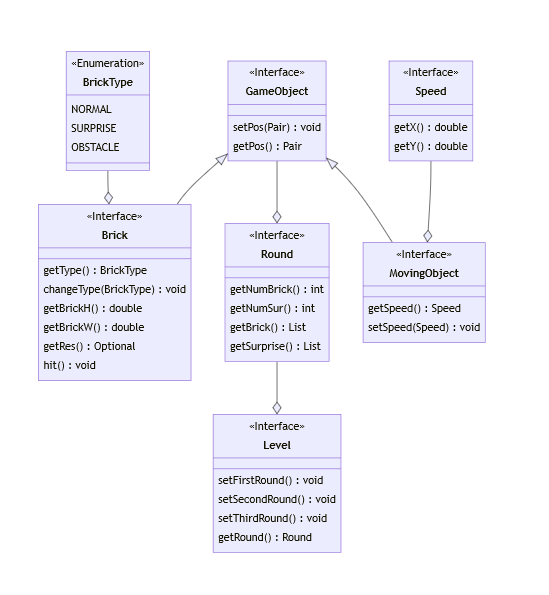
\includegraphics[scale=0.8]{images/analysis.png}
    \caption{Schema UML dell'analisi del problema, con rappresentate le entità principali ed i rapporti fra loro.}
    \label{images:analysis}
\end{figure}
\chapter{Design}
\section{Architettura}
Si è optato per un pattern architetturale ispirato a un MVC(Model , View, Controller) in cui ci siamo impegnati il più
possibile a mantenere separati gli aspetti logici, di controllo e di grafica. Tuttavia non ne rispetta tutti i principi poiché nella classe GameEngine ci siamo
serviti di una funzionalità di una libreria grafica (SwingWorker).
\\La nostra strategia ha comunque il vantaggio che qualora fosse necessario cambiare l'interfaccia grafica
questo non causerebbe modifiche nelle classi di Model e Controller.
\begin{figure}[H]
    \centering{}
    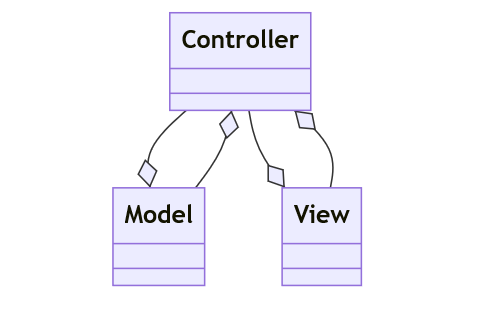
\includegraphics[scale=0.5]{images/MVC.png}
    \caption{Schema UML del pattern.}
    \label{images:MVC}
\end{figure}
Il pattern prevede comunque la suddivisione dei compiti in 3 parti:
\begin{itemize}
    \item Model gestisce i dati, la logica e le regole dell'applicazione.
    \item View responsabile della visualizzazione del dominio applicativo e dell'interazione con l'utente.
    \item Controller è l'elemento che si interporre tra il Model e la View.
\end{itemize}
Il Model è composto da varie classi e interfaccie che rappresentano i principali elementi applicativi (Level, Round, MovingObject, Brick, Pad, Surprise, SizeCalculation).
Di seguito nella \Cref{images:Model} seguente si può vedere una rappresentazione generale del Model.
\begin{figure}[H]
    \centering{}
    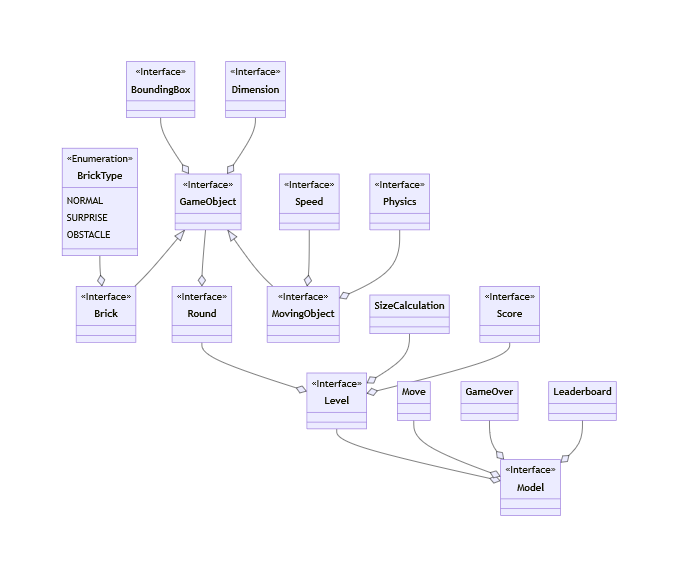
\includegraphics[scale=0.7]{images/Model.png}
    \caption{Schema UML del Model.}
    \label{images:Model}
\end{figure}
La View è gestita principalmente da un'interfaccia, UIController, che dirige tutti i vari JPanel (LeaderboardView, GameView, CommandsView, StartMenu) ed è colei
che comunica con il Controller dell'applicazione.
Vi è anche una classe astratta (AbstractView) che viene estesa dai vari menù di gioco (GameOver, PauseMenu e Victory) i quali utilizzano la classe CustomBtn
creata con lo scopo di avere i bottoni nei vari menù tutti con le stesse caratteristiche. Le principali dipendenze possono essere viste di seguito nella figura \Cref{images:View}.
\begin{figure}[H]
    \centering{}
    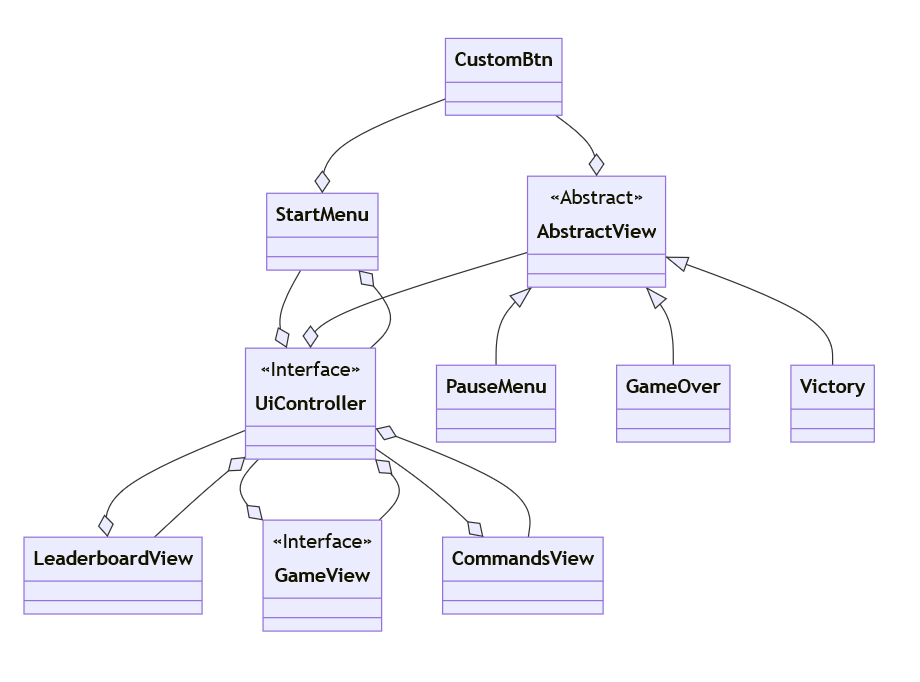
\includegraphics[scale=0.5]{images/View.png}
    \caption{Schema UML della View.}
    \label{images:View}
\end{figure}
Il Controller è costituito da una sola interfaccia che comunica con il Model e con la View ma anche con la classe GameEngine, il motore dell'applicazione.
\\Di seguito nella \Cref{images:Controller} l'UML del Controller.
\begin{figure}[H]
    \centering{}
    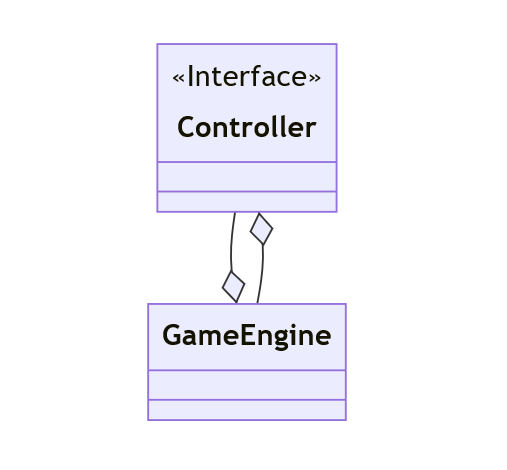
\includegraphics[scale=0.4]{images/Controller.png}
    \caption{Schema UML della View.}
    \label{images:Controller}
\end{figure}
\newpage
\section{Desing dettagliato}
\subsection{Ruggeri Simone}
Le parti di lavoro da me svolte hanno riguardato: la progettazione della struttura dei vari livelli,
l'impostazione del primo livello con i suoi 3 round, il controllo se il giocatore manca la pallina oppure se finisce il round, lo sviluppo di
alcuni metodi per i bonus, la parte di grafica che riguarda la pausa, il game over e la vittoria.\\\\
\textbf{Livelli}\\
Il gioco è suddiviso in tre livelli. Per la progettazione di una struttura comune per i livelli, ho creato un'interfaccia 'Level' e
un'abstract class 'AbstractLevel'. In Level vengono dichiarati i metodi che ogni livello dovrà possedere, mentre in AbstractLevel vengono implemetati. I metodi che
però definiscono caratteristiche differenti per ogni round del livello, sono dichiarati abstract e dovranno essere implementati nelle classi dei livelli. I tre livelli
dunque, 'FirstLevel','SecondLevel' e 'ThirdLevel', dovranno estendere la classe astratta AbstractLevel.
Level e AbstractLevel sono state create fin da subito, proprio per evitare di bloccare l'avanzamento dello sviluppo complessivo del progetto.
Inizialmente sono stati creati e implementati i metodi che avrebbero svolto le azioni principali, mentre successivamente a man mano che il progetto progrediva
sono stati aggiunti metodi e variabili che si sono dimostrati necessari.\\
Ogni livello è composto da tre round. Per quanto riguarda la realizzazione del primo livello, questi 3 round sono generati tramite delle costanti, che indicano
il numero di blocchi normali e blocchi sorpresa, da passare come argomento a 'RoundEasy'. RoundEasy definisce come questi blocchi debbano essere posizionati
nella schermata di gioco.
\begin{figure}[H]
    \centering
    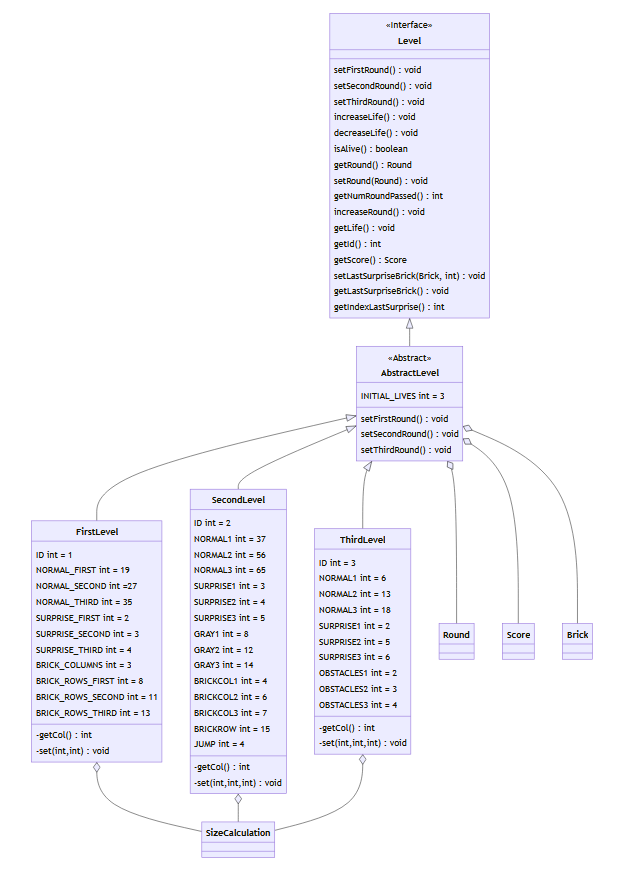
\includegraphics[scale=0.9]{images/Levels.png}
    \caption{Schema UML dell'organizzazione dei livelli.}
    \label{images:Levels}
\end{figure}
\newpage
\noindent
\textbf{Controlli sul Round}\\
Il decremento della vita all'interno del round di gioco e il passaggio all'eventuale round successivo sono
condizionati dai controlli fatti nella classe GameOver (del model). All'interno di questa classe sono presenti due metodi che restituiscono al Model
un valore booleano, che indicano se il player, tramite il controllo del pad, ha mancato la pallina oppure se il round è terminato.
\begin{figure}[H]
    \centering
    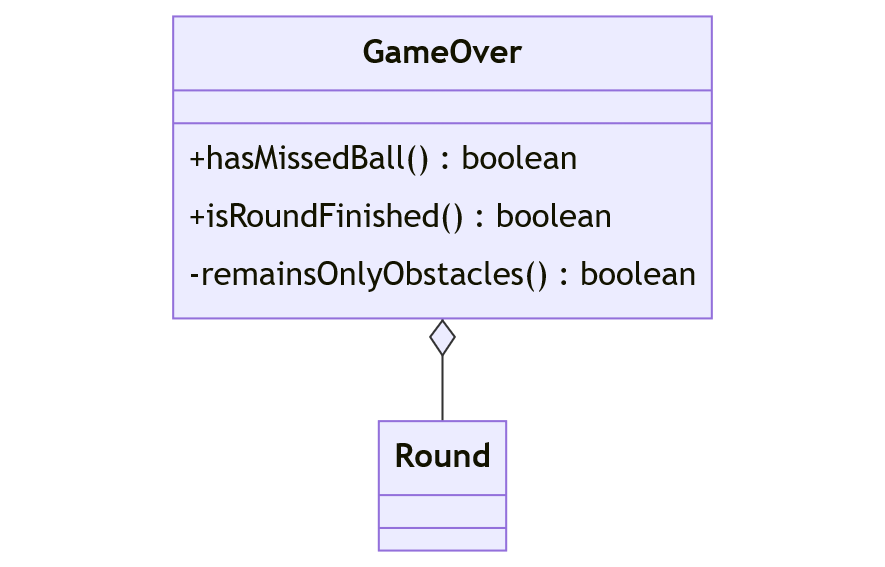
\includegraphics[width=0.8\textwidth]{images/GameOver.png}
    \caption{Schema UML della classe GameOver.}
\end{figure}
\noindent
\textbf{View di Pausa, Game Over e Vittoria}\\
La parte grafica del progetto prevede l'alternarsi di JPanels (che rappresentano menù inziale, menù di pausa, gameover, vittoria, classifica)
con la game view vera e propria.
Per la realizzazione della parte grafica di mia responsabilità (menù di pausa, game-over, vittoria), ho creato una classe astratta 'AbstractView'
che definsce delle impostazioni generali a cui fanno riferimento le classi che la estendono.
Queste caratteristiche prevedono uno sfondo nero, un titolo, e tre pulsanti. Due di questi pulsanti, menuBtn e quitBtn,
sono già definiti all'interno di AbstractView poichè sono in comune con tutti e tre i pannelli da visualizzare.
Il terzo pulsante viene impostato in AbstractView (a livello di posizionamento) ma definito nelle classi che estendono poichè questo pulsante e la
relativa azione che svolge cambia in base a quale panel l'untente si interfaccia nell'avanzamento del gioco.
L'istanza UIController permette ai pannelli di poter svolgere azioni come cambiare view (da tutti e tre i panels è possibile tramite il pulsante
mentuBtn andare alla schermata iniziale di gioco).
\begin{figure}[H]
    \centering
    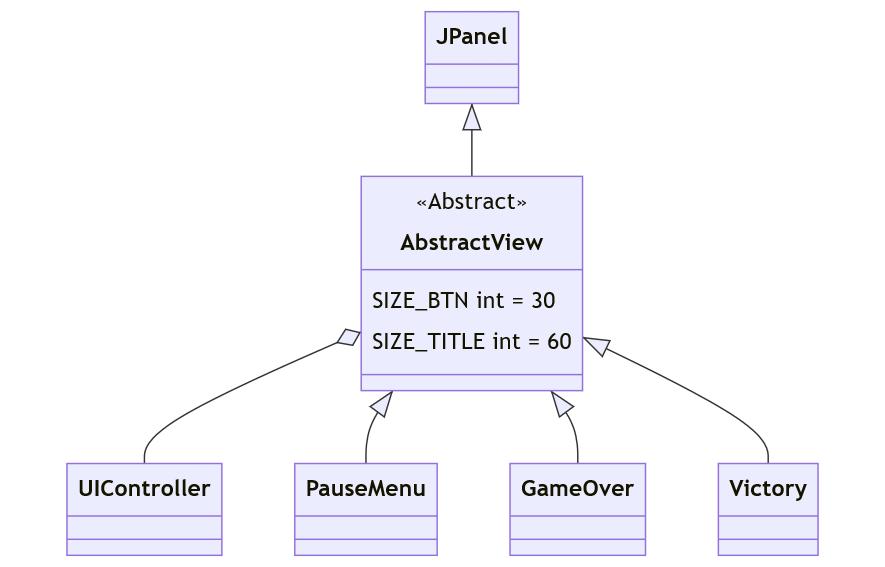
\includegraphics[width=0.8\textwidth]{images/AbstractView.png}
    \caption{Schema UML dell'implementazione della View di Pausa, Game Over e Vittoria.}
\end{figure}
\pagebreak
\subsection{Desiderio Edoardo}
Dal momento in cui si è formato il gruppo il mio primo obbiettivo è stato quello preoccuparmi di creare una buona impostazione,
in particolare grazie al colloquio con il professor Pianini ho potuto chiarire al gruppo in maniera definitiva come fosse meglio
lavorare sul repository del progetto e come doveva funzionare il pattern dell'applicazione da noi scelto.
In oltre, ho studiato come funzionano i file json di configurazione di vscode in maniera da fornire una configurazione user friendly
a tutti i miei colleghi per un' esperienza "out of the box" dell' IDE come la configurazione di un debugger meno invasivo rispetto quello di  default.
Ho riservato una buona attenzione a questa configurazione per limitare al massimo lo stress causato dalla poca intuittività di alcune
automattizzazioni ed essere sereni e tranquilli.
\\\textbf{UIController, la scelta.}\\
ho ritenuto vantaggioso avere un controller dedicato per la vista  che comunicasse
con il controller principale dell' applicazione.

Pagando con una maggiore ripetizione dei metodi "messaggeri" che si occupano semplicemente di trasportare informazioni
dall' applicazione alla sua vista si ottiene una maggiore manutentibilità e scalabilità dell'applicazione.
Di fatto si è verificato che modifice come:
\begin{itemize}
    \item modifica alle classi delle view
    \item aggiunta metodi o relativa modifica
    \item aggiunta di intere view
\end{itemize}
si sono rilevate poco costose sia in termini logici, guardando l'interfaccia UIController è lampante come muoversi,
che in termini pratici, per aggiungere una nuova vista basta aggiungere la sua dichiarazione e il metodo che la invochi.
\begin{figure}[H]
    \centering
    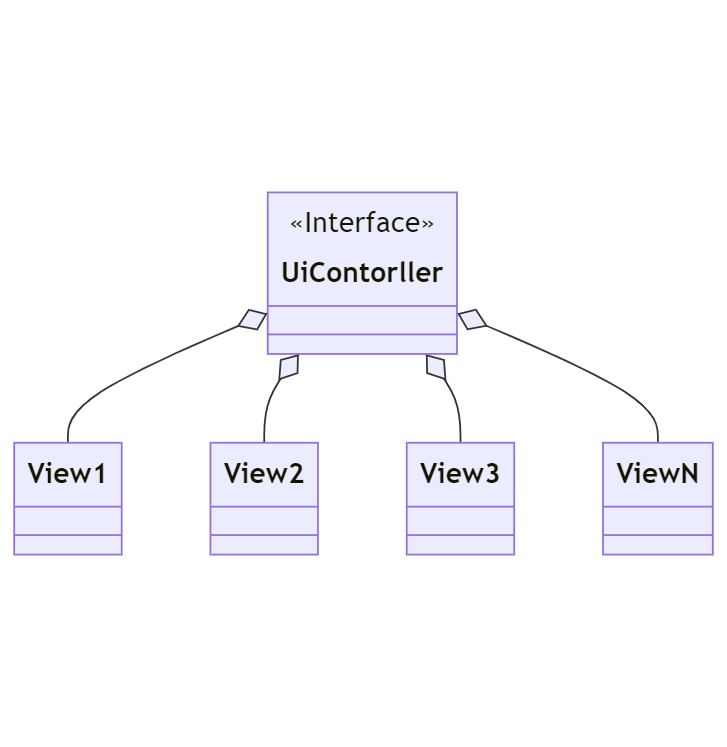
\includegraphics[width=0.8\textwidth]{images/UiControllerDesing.png}
    \caption{proiezione UML della comunicazione fra il controller principale e le viste con UIController}
\end{figure}

\textbf{UIController, l'implementazione.}\\
Per gestire le varie viste ho scelto di utilizzare un layout di jswing chiamato CardLayout.
Questo layout è funzionale a quello che intendevo far fare al View-controller poichè
gestisce due o più componenti che condividono lo stesso spazio di visualizzazione (il jframe nel nostro caso).

Ogni carta\footnote{nel nostro caso, classi che estendevano JPanel in modo da personalizzarne i meccanismi}
all'avvio dell' applicazione viene aggiunta al "deck"\footnote{il JPanel che riempie il frame principale}
a questo punto, con i metodi preposti al selezionamento di una carta basterà richiamarli per una visualizzazione
corretta.
Come sicuramente descritto anche dai miei colleghi, ogni classe View ha un riferimento all'interfaccia
del loro controller, di fatto il controller quindi "osserva" il comportamento della view e quando accade una
determinata interazione della stessa si scatenerà l'evento desiderato.
Per questo tipo di desing mi sono ispirato alle soluzioni viste in laboratorio e come mi è stato detto
a ricevimento questo modo di fare non è un pattern observer puro ma posso affermare che sia di simile
comportamento.

CardLayout non è oro colato, infatti se non fosse stato per l'attività di debugging non sarei mai riuscito
a capire che non cambia da solo il focus sulla finestra appena selezionata, risultava impossibile
inserire comandi input da tastiera se non dalla prima finestra aperta e la cosa é stata rislota
aggiornando il focus alla carta appena selezionata.\\

\textbf{Window resizable.}\\

l'idea nasce con la logica di mantenere sempre fisse le dimensioni del model
e di renderizzare la view in maniera tale da crearne semplicemente le loro proiezioni su schermo.
\begin{figure}[H]
    \centering
    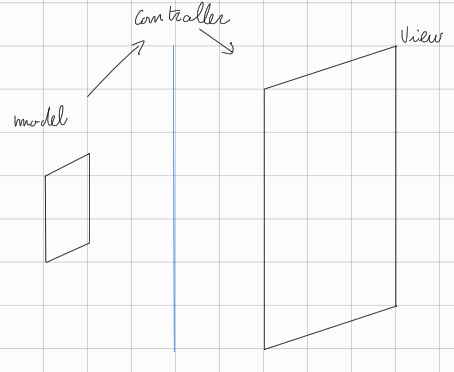
\includegraphics[width=0.8\textwidth]{images/resizableConcept.png}
    \caption{bozza della proiezione di un mattoncino fatta durante lo studio}
\end{figure}
l'implementazione segue la logica descritta in figura: il model passa gli oggetti da disegnare con le
relative dimensioni e posizioni sul paino, é compito poi del controller filtrarle e restituirle alla view,
ricarlcolate in maniera opportuna.\\
\textbf{Window resizable, la proporzione}\\
per proiettare correttamente gli oggettti di dimensione del model il controller deve moltiplicare ognuno
di questi per un delta di proiezione.

Questo Delta é calcolato facendo il rapporto fra quelle che sono le dimensioni correnti della View , rispetto
a quelle del model.\\
\textbf{esempio:} \\
assumiamo ipoteticamente che le dimensioni del model siano un mondo 400x400 nel quale sia disposto un mattoncino
con coordinate (2,3) e lunghezza e altezza (5,2).
A run time la view ha dimensioni 800x800  e quindi il controller posizionerá il mattoncino seguendo la logica
sopra descritta.\\
\begin{itemize}
    \item calcolo $\Delta W \rightarrow$  800/400 = 2
    \item calcolo $\Delta H \rightarrow$  800/400 = 2
    \item calcolo coordinate $\rightarrow P(2 \times \Delta W, 3\times \Delta H)$
    \item calcolo dimensioni $\rightarrow Dim(5 \times \Delta W,2\times \Delta H)$
\end{itemize}
in questa maniera viene assicurato un giusto mantenimento delle proporzioni delgi spazi decisi nel model.
Utilizzando questo tipo di proiezione assicuro anche il fatto che qualsiasi evento generato nel model, come una
collisione fra oggetti, venga riprodotto fedelmente sulla view.


\pagebreak
\subsection{Castiglioni Chiara}
Nel corso dello sviluppo del progetto mi sono occupata principalmente della parte riguardante la struttura dei vari round, il game loop del videogioco,
la parte di calcoli per il posizionamento delle varie entità e della loro diminsione, lo sviluppo di due metodi per i bonus, la creazione dell'entità Brick
mentre nella parte della View l'apparizione della scritta che indica il bonus preso.\\Inoltre ho collaborato con i miei compagni nell'implementazione delle parti comuni come
il Controller oppure il Model.\\
\textbf{GameEngine}
\\Questa classe è il vero e proprio motore del gioco al cui interno vi è il game loop cioè un ciclo che viene attivato quando:
\begin{itemize}
    \item L'utente seleziona uno dei tre livello messi a disposizione nello StartMenu.
    \item Si riprende il gioco dal menù di pausa.
    \item Si inizia un nuovo round.
\end{itemize}
mentre invece viene interrotto nel momento in cui:
\begin{itemize}
    \item Viene aperto il menù di pausa all'interno della partita.
    \item Il giocatore perde le sue tre vite messe a disposizione.
    \item L'utente vince il round e deve passare a quello successivo.
    \item Il giocatore vince la partita.
\end{itemize}
Per la realizzazione del game loop mi sono servita di una classe della libreria Swing cioè SwingWorker che consente di eseguire un thread in background
in quanto Swing utilizza un singolo thread cioè Event dispatch thread.
\\All'interno del game loop richiamo alcuni metodi privati che richiamano a loro volta metodi del Controller in quanto questa classe deve comunicare con il Model
e con la View aggiornandoli continuamente.
\\Per quanto riguarda l'aggiornamento del Model il game loop si occupa continuamente di:
\begin{itemize}
    \item Richiamare l'update delle entità in movimento.
    \item Controllare se vi è la terminazione del round e in tal caso richiamare l'inizializzazione del round successivo se vi è, altrimenti, viene impostata la vittoria.
    \item Controllare il meccanismo di perdita di vita dell'utente, nel caso avesse ancora vite viene riposizionata la pallina alla posizione iniziale altrimenti viene dichiarato game over.
\end{itemize}
In riferimento alla View il game loop si occupa di richiamare la repaint del Frame.
\\All'interno della classe GameEngine vi è anche un metodo che viene richiamato come ultimo all'interno del ciclo che si occupa di mantenere
la stessa velocità di esecuzione del ciclo su diversi PC in modo tale da evitare che su dispositivi molto prestanti l'applicazione venga eseguita troppo velocemente.
\begin{figure}[H]
    \centering{}
    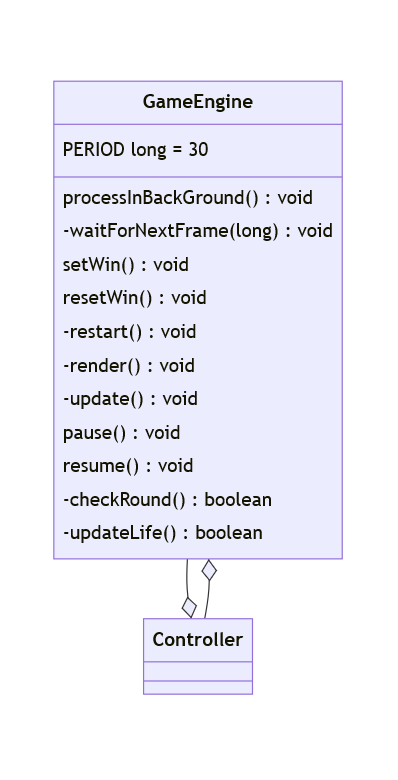
\includegraphics[scale=0.5]{images/GameEngine.png}
    \caption{Schema UML del GameEngine.}
    \label{images:GameEngine}
\end{figure}
\textbf{Brick}\\
Fin da subito mi sono occupata dell'entità brick facendo un'interfaccia Brick che estende quella già implementata dai miei colleghi (GameObject) in modo tale da avere già i metodi
per la posizione dei brick, la loro boundingBox e la loro dimensione.
\\Per questa entità ho poi implementato una classe astratta che implementa l'interfaccia in modo tale che le due diverse tipologie di blocchi (normali e ostacoli) potessero estenderla ereditando dei medoti
già implementati come per esempio il tipo di blocco e tutti i metodi dell'interfaccia GameObject, al fine di poter un giorno estendere i tipi di blocchi, mentre altri, invece, da implementare in quanto differiscono dalle diverse tipologie di blocchi.
In particolare mi sono occupata della classe NormalBrick che estende AbstractBrick la quale si occupa delle creazione di blocchi normali oppure hard a seconda della resistenza datagli.
\\Questa scelta strutturale è dovuta dal fatto che i brick normali e quelli hard differiscono solamente a livello della quantità di resistenza quindi, ho ritenuto inutile creare un'altra classe e
aggiungere un tipo diverso di brick all'interno di BrickType.
\begin{figure}[H]
    \centering{}
    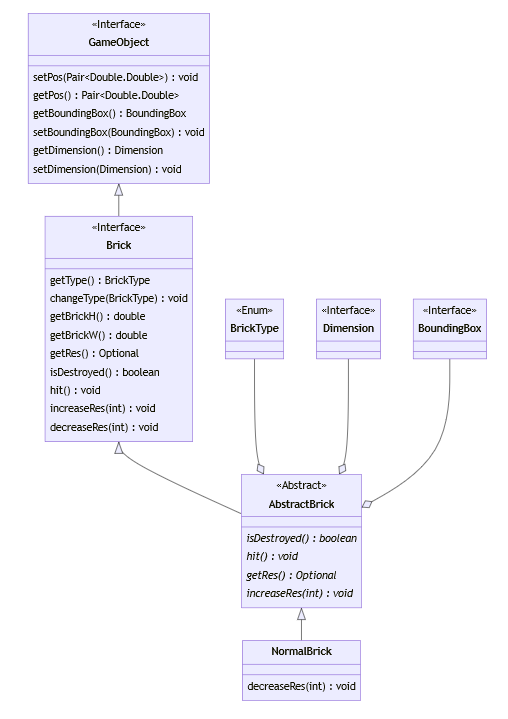
\includegraphics[scale=0.6]{images/Brick.png}
    \caption{Schema UML dell'entità brick.}
    \label{images:Brick}
\end{figure}
\textbf{SecondLevel}\\
In questa classe mi sono occupata principalmente della scelta sulla quantità di blocchi da disporre all'interno dei tre round. La struttura della mia classe può essere
visualizzata alla \Cref{images:Levels}.\\
\textbf{SizeCalculation}\\
Questa classe si occupa di eseguire calcoli riguardanti il posizionamento delle varie entità e la loro dimensione all'interno del mondo di gioco al
quale abbiamo deciso di dargli una dimensione fissa.
\\L'idea che mi era venuta in mente era quella di calcolare le dimensioni del brick in base al numero di brick da posizionare, mentre di lasciare mezza lunghezza di brick dai rispettivi
lati del mondo per calcolare il punto di partenza e di fine del posizionamento dei blocchi lungo l'asse delle ascisse. Per il calcolo dell'ordinata invece viene calcolata in base al numero di brick per colonna,
questo perché ogni round ha sempre più blocchi quindi necessita di spazio maggiore.
\\Vi sono anche due metodi che calcolano le dimensioni del pad e della pallina rispetto alle dimensioni del mondo nel model e un metodo che serve alla view per sapere qual è
la coordinata y di ogni riga in modo da riuscire a colorare in modo diverso ogni riga.
\begin{figure}[H]
    \centering{}
    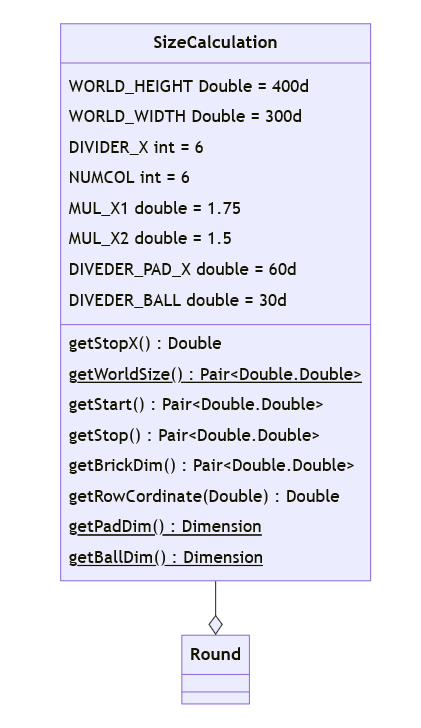
\includegraphics[scale=0.5]{images/SizeCalculation.png}
    \caption{Schema UML di SizeCalculation.}
    \label{images:SizeCalculation}
\end{figure}
\textbf{Round}\\
Per quanto riguarda l'organizzazione dei vari round è stato utile fin da subito creare una classe astratta in quanto ha permesso ai miei colleghi di estenderla e creare il proprio round e permetterà in futuro
di aggiungerne altri.
\\All'interno di questa classe ho scelto di implementare i metodi utili per rimuovere i brick, per settare i brick surprise in modo randomico, in quanto
comune a tutti i tipi di round, il metodo per aggiungere le palline surprise e altri metodi get e set.
\\L'unico metodo che ho deciso di mettere abstract è quello per il posizionamento dei brick in quanto ogni livello ha un proprio
round con una diversa disposizione.\\
\textbf{Round Medium}
\\Il round al quale mi sono dedicata io stessa è quello medio dove la disposizione dei brick è composta
da tre colonne separate ognuna con quattro blocchi ciascuna e vi è una tipologia di blocco in più rispetto agli altri cioè quello hard.
La differenza tra i tre round all'interno del mio livello è che il numero di righe e il numero di brick hard e brick surprise aumentano.
\\All'interno di questa classe ovviamente ho implementato il metodo che era definito astratto dove all'interno
richiamo anche i metodi per posizionare i blocchi surprise e quelli hard in modo randomico. Per posizionare i brick ovviamente mi sono servita
della classe SizeCalculation già descritta per sapere dove partire a inserirli.
\begin{figure}[H]
    \centering{}
    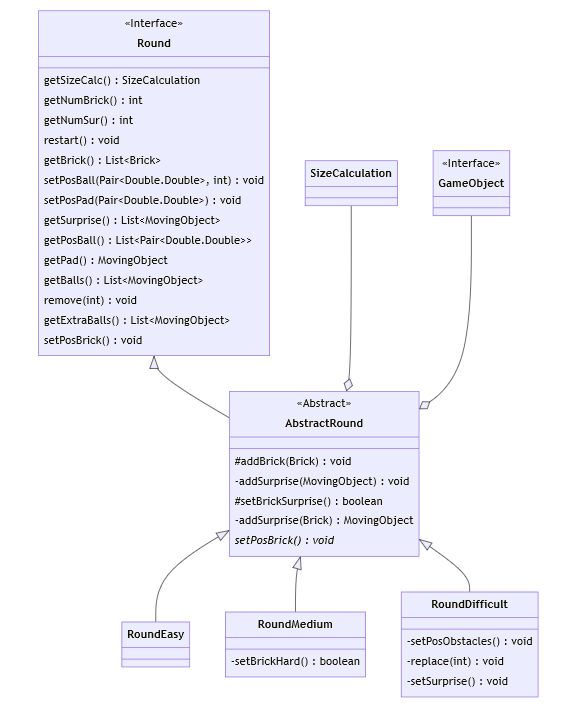
\includegraphics[scale=0.65]{images/Round.png}
    \caption{Schema UML della struttura Round.}
    \label{images:Round}
\end{figure}
\textbf{Bonus}\\
In questo progetto mi sono anche dedicata a creare due bonus che fossero correlati con quello che ho spiegato fino ad ora, cioè i blocchi hard.
\\Infatti i miei due surprise sono uno un bonus in quanto cambia per 10 secondi i blocchi hard con quelli normali mentre l'altro è un malus perché aggiungo una riga di
blocchi hard. Per l'implementazione del primo mi sono servita di due classi di libreria Timer e TimerTask, sovvrascrivendo il metodo run che è colui che scaduto il Timer
esegue le istruzioni che ha al suo interno.

\pagebreak
\subsection{Foschi Virginia}
Nel corso dello sviluppo del progetto il mio lavoro si è principalmente concentrato sulla gestione e implementazione della classifica di gioco, del salvataggio del punteggio, del livello difficile con i corrispondenti round e della visualizzazione dei comandi principali del gioco.\\
Tuttavia ho collaborato anche alla creazione dei bonus e alla visualizzazione degli oggetti del gioco.\\\\
\textbf{Classifica di gioco}\\
Per quanto riguarda la realizzazione della classifica ho optato per la creazione, all'avvio dell'applicazione, di un file di testo nella home directory dell'utente in cui verrranno inizialmente caricati i punteggi conseguiti da me e i miei compagni che si trovano memorizzati all'interno di un file di testo nella cartella resources del progetto.
\\Ogni giocatore ha la possibilità, una volta completato il livello o dopo aver perso, di memorizzare il punteggio complessivo conseguito inserendo nome e password. Si è pensato infatti all'utilizzo di una password in modo da permettere al giocatore, una volta riaperta l'applicazione, di aggiornare il punteggio conseguito nelle partite precedenti.
\\La memorizzazione del punteggio avvine nel seguente modo:
\begin{itemize}
    \item Ogni volta che il giocatore decide di salvare il punteggio conseguito in un determinato livello, il vecchio punteggio, relativo a quel livello, sarà sempre rimpiazzato dal nuovo.
    \item Il punteggio complessivo, cioè quello visualizzato nella classifica, sarà dato dalla somma dei punteggi conseguiti nei 3 livelli.
\end{itemize}
La classifica aggiornata è in ogni momento visualizzabile cliccando l'apposito tasto presente nel menù di gioco.\\\\
\begin{figure}[H]
    \centering{}
    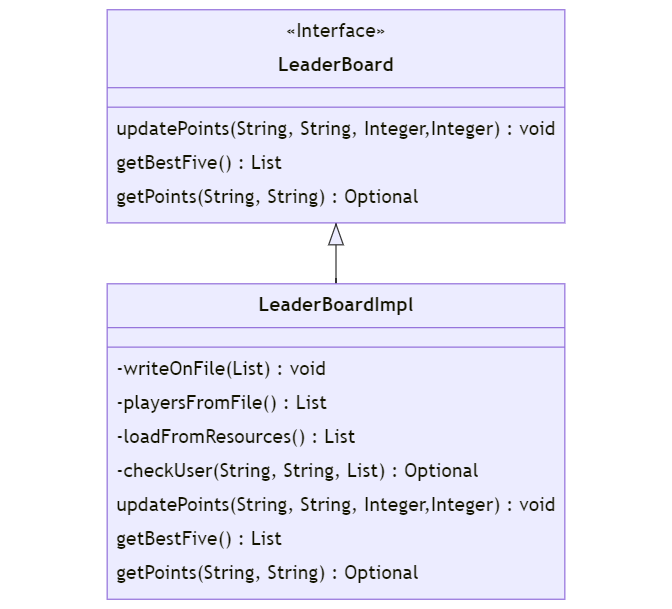
\includegraphics[scale=0.4]{images/leaderboard.png}
    \caption{Schema UML della leaderboard.}
    \label{images:leaderboard}
\end{figure}

\textbf{Livello e round difficile}\\
Per quanto riguarda invece la struttura dei livelli e dei round si è cercato di organizzare il tutto in modo tale da creare codice facilmente espandibile in caso di aggiunta di ulteriori livelli di gioco e round.
\\Ogni livello mantiene informazione sul round corrente al cui interno sono contenute tutte le informazioni riguardanti gli oggetti in gioco con le corrispondenti caratteristiche (posizione, velocità, dimensione,...).
In particolare il livello difficile è caratterizzato dalla presenza di ostacoli, cioè mattoncini indistruttibili, e dalla disposizione dei blocchi in maniera piramidale.
\\Mi sono basata sulla strutturazione e organizzazione delle classi realizzata dai miei compagni, che è possibile osservare in maniera dettagliata alla \Cref{images:Levels} e \Cref{images:Round}, e mi sono occupata del collegamento tra le varie classi in modo da permettere la visualizzazione a video degli oggetti del gioco tramite la classe GameView.\\\\


\pagebreak

\textbf{View}\\
Dal punto di vista della view mi sono occupata principalmente dell'implementazione di 3 interfacce grafiche:\\
\begin{itemize}
    \item LeaderBoardView: interfaccia che permette di visualizzare a video la classifica costituita dai migliori 5 giocatori.
    \item CommandView: insieme ai miei compagni abbiamo pensato di realizzare un'interfaccia per permettere al giocatore di visualizzare i comandi principali del gioco.
    \item SaveScore: JDialog che permette al giocatore di inserire i suoi dati (nome e password) e salvare il proprio punteggio.
\end{itemize}
\pagebreak
\subsection{Balzoni Margherita}
Il mio contributo all'interno del progetto ha riguardato principalmente la gestione della fisica della pallina, in particolare gli aspetti di creazione delle BoundigBox, controllo delle collisioni, movimento e gestione della direzione della palla.
\\Mi sono occupata poi di realizzare il menù iniziale di gioco e implementare la classe che memorizza e increamenta il punteggio durante la partita.
\\Ho inoltre collaborato alla realizzazione di alcuni bouns, nello specifico l'aggiunta di una pallina extra e il raddoppio del punteggio per un determinato periodo di tempo.\\\\
\textbf{BoundigBox}\\
Per delimitare l'area occupata dai vari oggetti di gioco ho utilizzato una Bounding Box, ovvero il più piccolo rettangolo capace di contenere una determinta figura al suo interno.\\
Sono partita realizzando un'intefaccia BoundigBox la quale viene implementata da una classe astratta AbstractBoundingBox.
Successivamente ho creato due classi, CircleBoundingBox e RectBoundingBox, che estendono la classe astratta. In particolare la prima permette la creazione di Bounding Box per gli oggetti circolari come le palline e gli oggetti surprise, mentre la seconda le realizza per il pad e i brick.
\\La box viene creata grazie ad una mappa all'interno della quale sono memorizzate le coordinate di tutti e quattro gli angoli della "scatola".
\\Il metodo collideWith all'interno implementato all'interno della classe astratta AbstractBoundigBox permette di verificare l'intersezione tra due bounding box, se ciò non avviene verrà restituito un opzionale vuoto, in caso contrario restituirà il punto in cui è avvenuta la collisione:
\begin{itemize}
    \item  Su uno dei due lati orizzontali della box.
    \item  Su uno dei due elati verticati della box .
    \item  Tra due angoli della box .
  
\end{itemize}
Questa informazine ci sarà utile in seguito per verificare le collisioni e gestire il cambio di direzione della palla.
\begin{figure}[H]
    \centering{}
    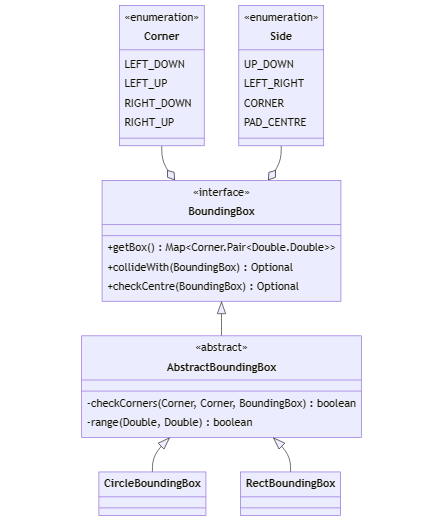
\includegraphics[scale=0.6]{images/BoundingBox.png}
    \caption{Schema UML della BoundigBox.}
    \label{images:BoundigBox}
\end{figure}
\textbf{Gestione della direzione}\\
\begin{figure}[H]
    \centering{}
    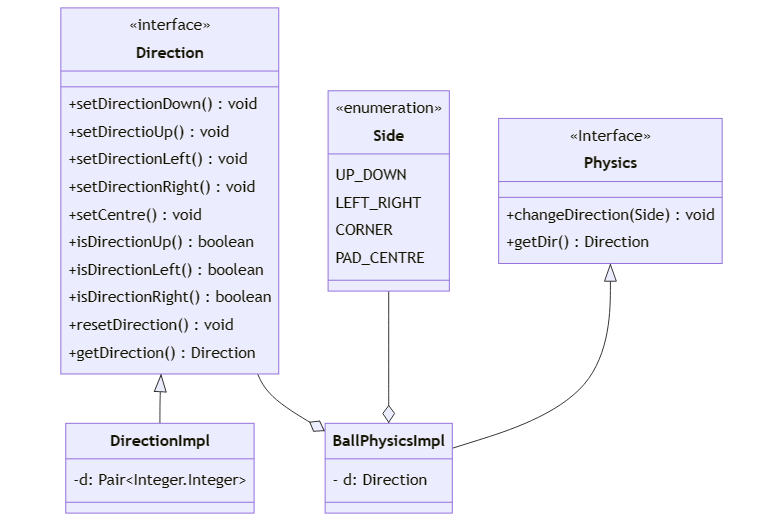
\includegraphics[scale=0.6]{images/Physics.png}
    \caption{Schema UML della gestione della direzione.}
    \label{images:Physics}
\end{figure}
\textbf{Collisioni}\\
\begin{figure}[H]
    \centering{}
    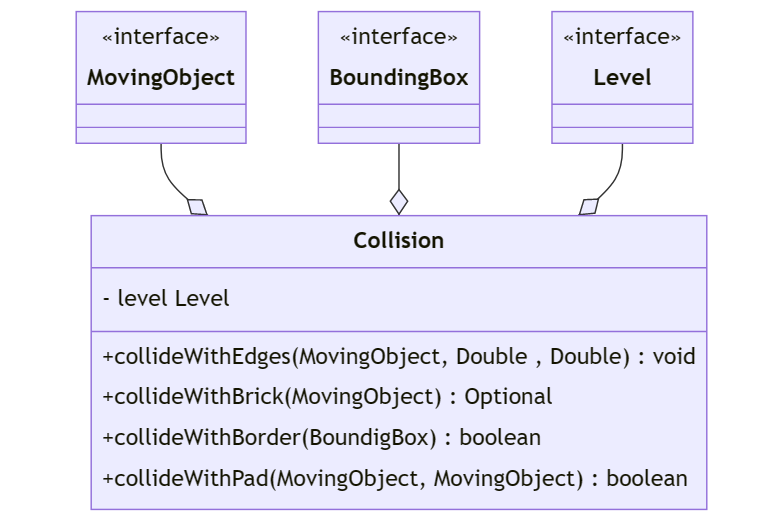
\includegraphics[scale=0.6]{images/Collision.png}
    \caption{Schema UML della gestione delle Collisioni.}
    \label{images:Collision}
\end{figure}
\textbf{Movimento}\\
\begin{figure}[H]
    \centering{}
    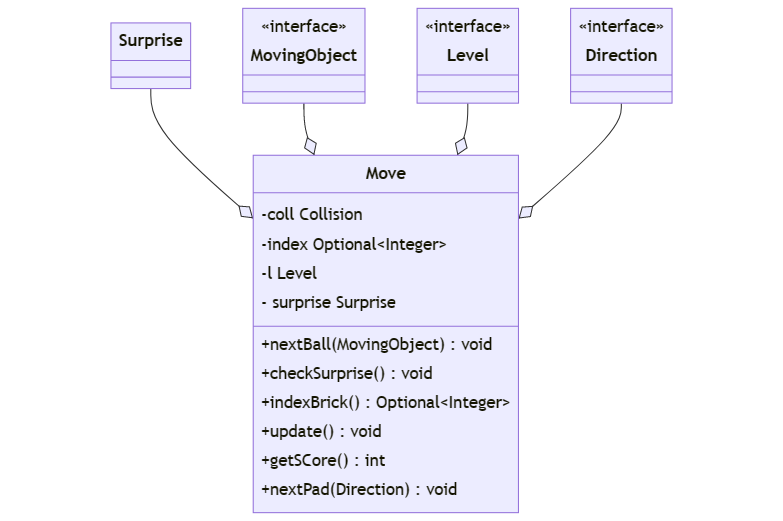
\includegraphics[scale=0.6]{images/Move.png}
    \caption{Schema UML del Movimento.}
    \label{images:Move}
\end{figure}
\textbf{Punteggio}\\
\begin{figure}[H]
    \centering{}
    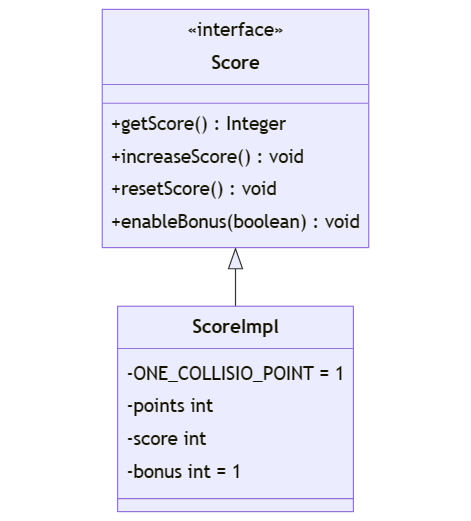
\includegraphics[scale=0.6]{images/Score.png}
    \caption{Schema UML del Punteggio.}
    \label{images:Score}
\end{figure}
\pagebreak
\chapter{Sviluppo}
\section{Testing automatizzato}
In parallelo allo sviluppo del progetto sono stati effettuati anche diversi test automatici utilizzando la libreria JUnit.
Sulle componenti principali sono stati eseguiti i seguenti test automatici:
\begin{itemize}
    \item Test sui bonus: abbiamo scelto di testare ognuno i propri bonus all'interno dei vari livelli.
    \item Test sulla entità brick: testato la resistenza di un blocco hard e degli ostacoli.
    \item Test sulle modalità di game over.
    \item Test sulla classifica: si verifica la correttezza del salvataggio del punteggio del giocatore.
    \item Test sulla dinamica: sulle collisioni e sul movimento dei MovingObject.
\end{itemize}
Si è anche dedicato del tempo fer fare dei test manuali dedicati principalmente al ridimensionamento della finestra di gioco.
Il gioco è stato collaudato su più sistemi operativi:
\begin{itemize}
    \item Windows 10 e 11.
    \item Light Ubuntu 22.04.1.
    \item macOS.
\end{itemize}

\section{Metodologia di lavoro}
Per lavorare
a questo progetto abbiamo cercato di strutturare il lavoro seguendo queste macro domande:
\subsubsection{Qual'è la missione del progetto e con quali risorse si intende perseguirla?}
La missione del progetto è ampiamente descritta nei paragrafi precedenti.
Le risorse da noi scelte in fase di pianificazione e progettazione sono varie tra cui:
\begin{itemize}
    \item materiale didattico fornito dai professori
    \item plugin gradle
    \item versione di java 17
    \item git e github\footnote{\url{github.com}}
    \item strumenti di pianificazione, comunicazione e in generale multimediali forniti dall'account aziendale (unibo).
\end{itemize}

\subsubsection{Come verrà condotto il progetto?}
Si può riassumere la conduzione del progetto con un'organigramma orizzontale.
Ognuno ha piena responsabilità dei compiti che ci si è auto affidato al tempo di decisione e assegnazione delle task.
Questo implica il fatto che l'auto organizzazione di ogni singolo componente è fondamentale per la buona riuscita del progetto.
Ovviamente in caso di difficoltà il gruppo stimolerà il singolo a una soluzione senza però intaccarne la creatività.
\subsubsection{Come ne verrà controllato l'avanzamento?}
\subsubsection{Organizzazione DVCS}
Nelle varie risorse scelte sono indicati git e github, git è un software DVCS presentato e spiegato a lezione mentre github.com è un servizio
hub di repository.
La produzione è organizzata su più branch.
\\Il branch principale (master nel nostro caso) raccoglie tutto il codice di progetto approvato da tutti, su github è settata una policy
di sicurezza affinchè sia obbligatorio aprire una pull request per poter eseguire il merging del codice.
Il branch develop raccoglie la linea di sviluppo in fase di pre-relies in cui è ammissibile trovare eventuali bug o errori di desing.
\\Ogni elemento del teamWork, ad ogni step evolutivo, si occupa di creare un branch locale che non è necessario venga pubblicato poichè finito
il lavoro si occuperà di eseguire il merging  in develop.
\subsubsection{Ciclo di vita del progetto}
Ogni pull request (develop - master) verrà eseguita quando il codice develop soddisfa i requisiti che l'applicazione deve avere rispetto
all'obbiettivo incrementale che ci siamo posti.
In linea di massima la nostra scelta è di procedere a piccoli passi fino alla finalizzazione del progetto.\\
\\La parte di lavoro sviluppata in comune è stata quella inanzitutto della parte di analisi iniziale e poi successivamente durante il corso dello sviluppo
sono state implementate classi comuni a tutti come quelle del Controller e quelle del Model, dove ognuno ha inserito dei metodi che servivano per collagare
le parti di codice già create singolarmente.
\\Si riporta di seguito la divisione dei compiti di ogni componente del gruppo.
\subsection{Castiglioni Chiara}
Le attività da me svolte sono state:
\begin{itemize}
    \item Creazione della struttura dei round e il relativo round medio.
    \item Gestione del game loop.
    \item Implementazione della parte di calcoli riguardante la dimensione e posizione delle entità.
    \item Implementazione di due metodi all'interno della classe Surprise.
    \item Implementazione del livello medio.
    \item Creazione dell'entità brick.
    \item Apparizione della scritta al centro del frame che indica il bonus preso.
    \item Colorazione delle righe di brick.
\end{itemize}
\subsection{Foschi Virginia}
I compiti da me sviluppati sono stati:
\begin{itemize}
    \item Implementazione del livello difficile con i corrispondenti 3 round.
    \item Gestione classifica e salvataggio punteggio.
    \item Implementazione di 3 metodi all'interno della classe surprise.
    \item Visualizzazione degli oggetti (pad, pallina e brick) nella scena.
    \item Creazione e gestione delle palline bonus.
    \item Creazione e gestione degli ostacoli.
\end{itemize}
\subsection{Balzoni Margherita}
I compiti da me svolti sono stati:
\begin{itemize}
    \item Gestione della direzione della pallina.
    \item Creazione delle BoundigBox.
    \item Gestione delle collisioni della pallina con i bordi, il pad e i brick.
    \item Gestione del movimento della palla.
    \item Implementazione di due metodi della classe Surprise.
    \item realizzazione del menù iniziale dell'applicazione.
    \item Gestione del punteggio.
\end{itemize}

\section{Note di sviluppo}
In questa sezione vengono elencati gli aspetti avanzati del linguaggio utilizzato e di librerie.
\subsection{Desiderio Edoardo}
\begin{itemize}
    \item Ispirato dalla programmazione funzionale ho cercato di evitare il piú possibile la scrittura di switch
          statement all'interno del progetto, in questo snippet\footnote{\url{https://pastecode.io/s/18uxzd1a}} ho cercato
          di fare un esempio per tutti i compagni del gruppo. Adottare questo metodo garantisce di mantenere in ordine il codice
          e averne una manutentibilità e flessibilitá maggiore (la classe Surprise.java con uno switch sarebbe stata incomprensibile a mio avviso)
    \item utilizzo di CompletableFuture per rendere asicrone operazioni dei surprise in modo che impattino il meno possibile
          sull'esecuzione dell'intera applicazione
    \item tutte le collezioni che dovevo ricalcolare nel controller per rendere le figure resizable le ho modificate
          utilizzando stream combinate con lambda expression, l'utilizzo di lambda é stato fatto  anche in assenza di stream
\end{itemize}
\subsection{Foschi Virginia}
Nelle parti di codice da me curate, ho cercato, dove possibile, di fare uso delle seguenti funzionalità del linguaggio Java:
\begin{itemize}
    \item uso di stream e lambda expression dove possibile per rendere il codice più leggibile.
    \item Optional che mi hanno permesso di memorizzare tutti i mattoncini, indipendentemente dal tipo, in un'unica lista all'interno della classe round.
    \item Iterator per scorrere la lista delle palline bonus e contemporaneamente eliminarle in caso di contatto con il pad o fuoriuscita dal frame.
    \item java.util.Serializable per memorizzare l'oggetto User nel file.
\end{itemize}
\subsection{Castiglioni Chiara}
Nelle mia parte di progetto ho cercato di utilizzare il più possibile:
\begin{itemize}
    \item stream e lambda expression.
    \item Optional utilizzati per la resistenza dei brick.
    \item javax.swing.SwingWorker\footnote{\url{https://docs.oracle.com/javase/7/docs/api/javax/swing/SwingWorker.html}} per la realizzazione del game loop.
    \item java.util.Timer\footnote{\url{https://docs.oracle.com/javase/7/docs/api/java/util/Timer.html}} e java.util.TimerTask\footnote{\url{https://docs.oracle.com/javase/7/docs/api/java/util/TimerTask.html}} per l'implementazione di un metodo bonus e per l'apparizione della scritta del bonus preso.
\end{itemize}
L'unica fonte che ho utilizzato è stata {\url{https://www.youtube.com/watch?v=HUuiGW6TyfI}} per comprendere il funzionamento della
classe SwingWorker, oltre alla documentazione Oracle.

\chapter{Commenti finali}
\section{Autovalutazione e lavori futuri}

\appendix
\section{Guida utente}
All'avvio dell'applicazione si presenta la seguente schermata di menu iniziale:
\begin{figure}[H]
    \centering{}
    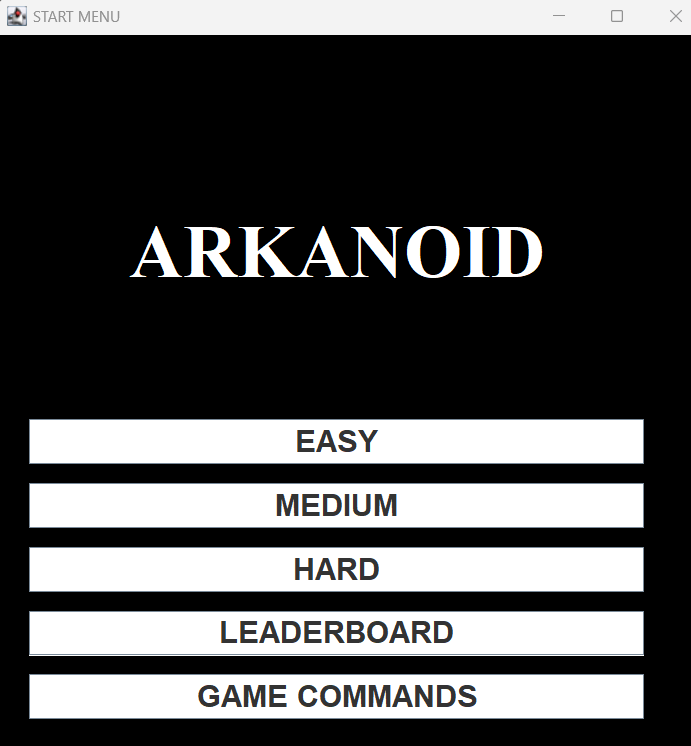
\includegraphics[scale=0.4]{images/StartMenuGuidaUtente.png}
    \caption{Schermata di menù iniziale.}
    \label{images:StartMenuGuidaUtente}
\end{figure}
Abbiamo 5 bottoni che hanno diverse funzionalità:
\begin{itemize}
    \item Premendo il pulsante EASY oppure MEDIUM oppure DIFFICULT si avvierà il gioco corrispondente alla difficoltà che viene selezionata.\Cref{images:Levels 2}
    \item Premendo il pulsante LEADERBOARD si potrà visionare la classifica.
    \item Premendo il pulsante GAME COMMANDS si potranno visionare i comandi di gioco.\Cref{images:Comandi}
\end{itemize}
\begin{figure}[H]
    \centering{}
    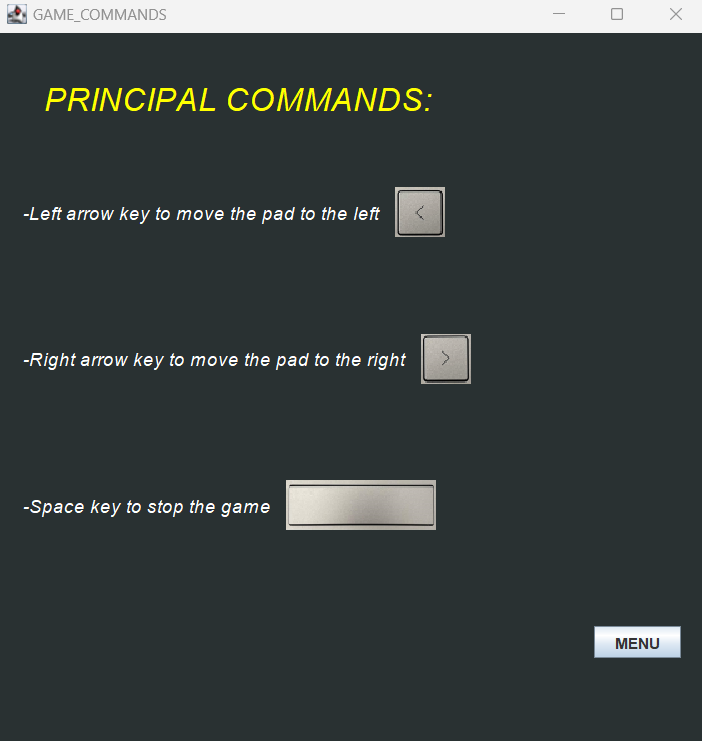
\includegraphics[scale=0.5]{images/GameCommandsGuidaUtente.png}
    \caption{Schermata dei comandi.}
    \label{images:Comandi}
\end{figure}
\begin{figure}[H]
    \centering{}
    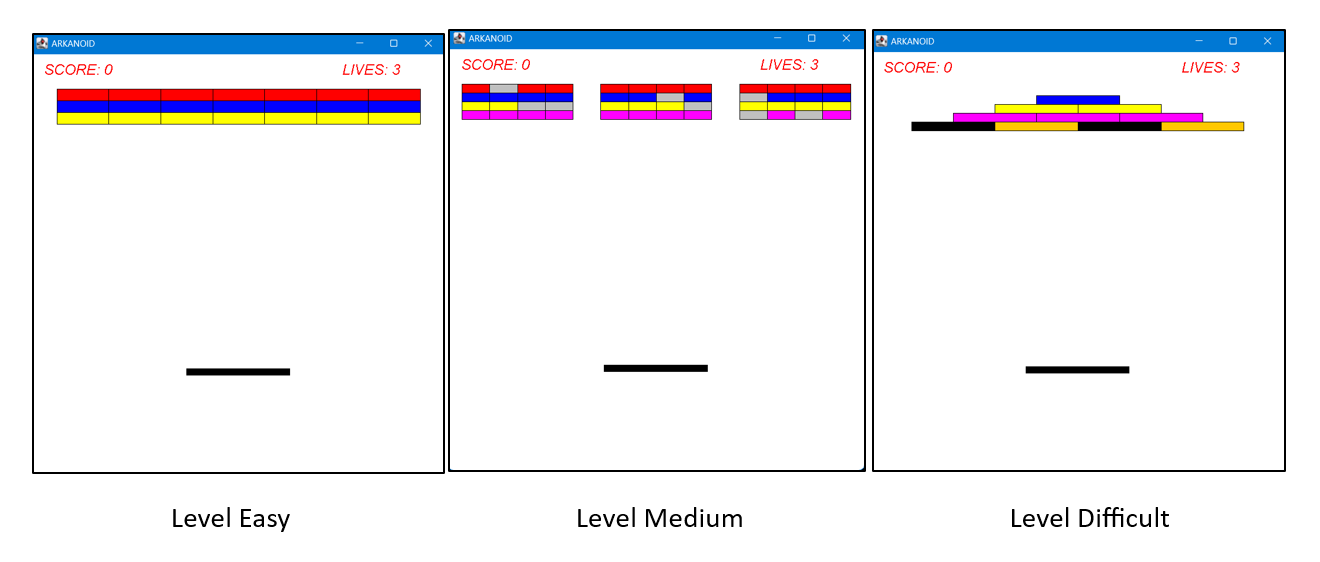
\includegraphics[scale=0.5]{images/Leves.png}
    \caption{Schermata dei tre livelli.}
    \label{images:Levels 2}
\end{figure}
Una volta premuto il livello desiderato, la schermata sarà una di questre tre \Cref{images:Levels}, in base al livello scelto,
e la pallina inizierà subito a muoversi.
\begin{figure}[H]
    \centering{}
    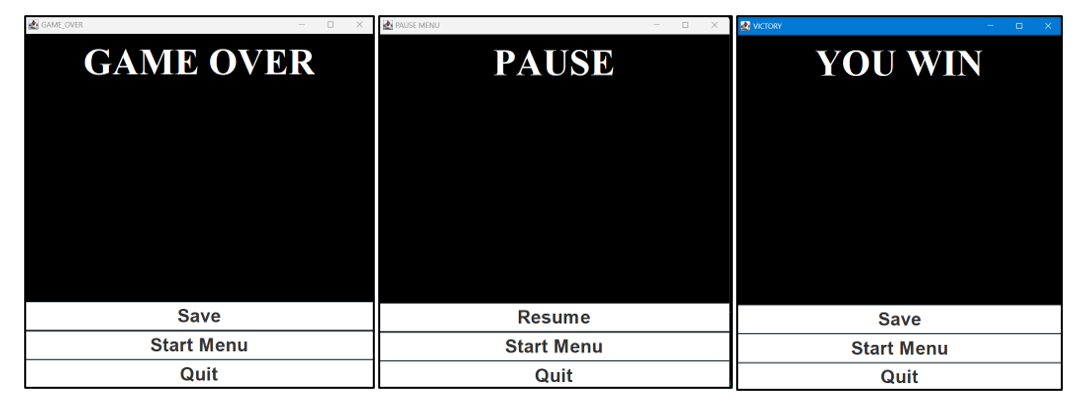
\includegraphics[scale=0.5]{images/Schermate.png}
    \caption{Schermate dei menù di pausa, gameover e vittoria.}
    \label{images:Views}
\end{figure}
Nei menù di GameOver e Victory si potrà scegliere se salvare il proprio punteggio,
ritornare al menù iniziale oppure uscire del tutto dall'applicazione. Stesse azioni sono
possibili farle nel menù di pausa ad eccezzione del pulsante save che viene sostituito da quello che
ha il compito di far ritornare l'utente alla partita in corso prima di averla stoppata (Resume).

\end{document}
